%----------------------------------------------------------------------------------------
%	PACKAGES AND OTHER DOCUMENT CONFIGURATIONS
%----------------------------------------------------------------------------------------

\documentclass[18pt]{extarticle}

%%%%%%%%%%%%%%%%%%%%%%%%%%%%%%%%%%%%%%%%%
% Lachaise Assignment
% Structure Specification File
% Version 1.0 (26/6/2018)
%
% This template originates from:
% http://www.LaTeXTemplates.com
%
% Authors:
% Marion Lachaise & François Févotte
% Vel (vel@LaTeXTemplates.com)
%
% License:
% CC BY-NC-SA 3.0 (http://creativecommons.org/licenses/by-nc-sa/3.0/)
% 
%%%%%%%%%%%%%%%%%%%%%%%%%%%%%%%%%%%%%%%%%

%----------------------------------------------------------------------------------------
%	PACKAGES AND OTHER DOCUMENT CONFIGURATIONS
%----------------------------------------------------------------------------------------

\setlength{\parindent}{0em}
\setlength{\parskip}{.5em}

\usepackage{amsmath,amsfonts,stmaryrd,amssymb} % Math packages

\usepackage{enumerate} % Custom item numbers for enumerations

\usepackage[ruled]{algorithm2e} % Algorithms

\usepackage[framemethod=tikz]{mdframed} % Allows defining custom boxed/framed environments

\usepackage{dirtytalk}

\usepackage{listings} % File listings, with syntax highlighting
\lstset{
	basicstyle=\ttfamily, % Typeset listings in monospace font
}

\usepackage{hyperref}
\hypersetup{
    colorlinks=true,
    linkcolor=blue,
    filecolor=magenta,      
    urlcolor=cyan,
}


%----------------------------------------------------------------------------------------
%	DOCUMENT MARGINS
%----------------------------------------------------------------------------------------

\usepackage{geometry} % Required for adjusting page dimensions and margins

\geometry{
	paper=a4paper, % Paper size, change to letterpaper for US letter size
	top=2.5cm, % Top margin
	bottom=3cm, % Bottom margin
	left=2.5cm, % Left margin
	right=2.5cm, % Right margin
	headheight=14pt, % Header height
	footskip=1.5cm, % Space from the bottom margin to the baseline of the footer
	headsep=1.2cm, % Space from the top margin to the baseline of the header
	%showframe, % Uncomment to show how the type block is set on the page
}

%----------------------------------------------------------------------------------------
%	FONTS
%----------------------------------------------------------------------------------------

\usepackage[utf8]{inputenc} % Required for inputting international characters
\usepackage[T1]{fontenc} % Output font encoding for international characters

\usepackage{XCharter} % Use the XCharter fonts

%----------------------------------------------------------------------------------------
%	COMMAND LINE ENVIRONMENT
%----------------------------------------------------------------------------------------

% Usage:
% \begin{commandline}
%	\begin{verbatim}
%		$ ls
%		
%		Applications	Desktop	...
%	\end{verbatim}
% \end{commandline}

\mdfdefinestyle{commandline}{
	leftmargin=10pt,
	rightmargin=10pt,
	innerleftmargin=15pt,
	middlelinecolor=black!50!white,
	middlelinewidth=2pt,
	frametitlerule=false,
	backgroundcolor=black!5!white,
	frametitle={Command Line},
	frametitlefont={\normalfont\sffamily\color{white}\hspace{-1em}},
	frametitlebackgroundcolor=black!50!white,
	nobreak,
	singleextra={%
    }
}

% Define a custom environment for command-line snapshots
\newenvironment{commandline}{
	\medskip
	\begin{mdframed}[style=commandline]
}{
	\end{mdframed}
	\medskip
}

%----------------------------------------------------------------------------------------
%	FILE CONTENTS ENVIRONMENT
%----------------------------------------------------------------------------------------

% Usage:
% \begin{file}[optional filename, defaults to "File"]
%	File contents, for example, with a listings environment
% \end{file}

\mdfdefinestyle{file}{
	innertopmargin=1.6\baselineskip,
	innerbottommargin=0.8\baselineskip,
	topline=false, bottomline=false,
	leftline=false, rightline=false,
    leftmargin=0cm,rightmargin=0cm,
	singleextra={%
		\draw[fill=black!10!white](P)++(0,-1.2em)rectangle(P-|O);
		\node[anchor=north west]
		at(P-|O){\ttfamily\mdfilename};
		%
		\def\l{3em}
		\draw(O-|P)++(-\l,0)--++(\l,\l)--(P)--(P-|O)--(O)--cycle;
		\draw(O-|P)++(-\l,0)--++(0,\l)--++(\l,0);
	},
	firstextra={%
		\draw[fill=black!10!white](P)++(0,-1.2em)rectangle(P-|O);
		\node[anchor=north west]
		at(P-|O){\ttfamily\mdfilename};
		%
	},
    middleextra={%
    },
    secondextra={%
		\def\l{3em}
		\draw(O-|P)++(-\l,0)--++(\l,\l)--(P)--(P-|O)--(O)--cycle;
		\draw(O-|P)++(-\l,0)--++(0,\l)--++(\l,0);
    },
    nobreak,
}

% Define a custom environment for file contents
\newenvironment{file}[1][File]{ % Set the default filename to "File"
	\medskip
	\newcommand{\mdfilename}{#1}
	\begin{mdframed}[style=file]
}{
	\end{mdframed}
	\medskip
}

%----------------------------------------------------------------------------------------
%	NUMBERED QUESTIONS ENVIRONMENT
%----------------------------------------------------------------------------------------

% Usage:
% \begin{question}[optional title]
%	Question contents
% \end{question}

\mdfdefinestyle{question}{
	innertopmargin=1.2\baselineskip,
	innerbottommargin=0.8\baselineskip,
	roundcorner=5pt,
	singleextra={%
		\draw(P-|O)node[xshift=1em,anchor=west,fill=white,draw,rounded corners=5pt]{%
		Άσκηση \theQuestion\questionTitle};
	},
	firstextra={%
		\draw(P-|O)node[xshift=1em,anchor=west,fill=white,draw,rounded corners=5pt]{%
		Άσκηση \theQuestion\questionTitle};
	},
}

\newcounter{Question} % Stores the current question number that gets iterated with each new question

% Define a custom environment for numbered questions
\newenvironment{question}[1][\unskip]{
	\bigskip
	\stepcounter{Question}
	\newcommand{\questionTitle}{~#1}
	\begin{mdframed}[style=question]
}{
	\end{mdframed}
	\medskip
}

%----------------------------------------------------------------------------------------
%	WARNING TEXT ENVIRONMENT
%----------------------------------------------------------------------------------------

% Usage:
% \begin{warn}[optional title, defaults to "Warning:"]
%	Contents
% \end{warn}

\mdfdefinestyle{warning}{
	topline=false, bottomline=false,
	leftline=false, rightline=false,
	nobreak,
	singleextra={%
		\draw(P-|O)++(-0.5em,0)node(tmp1){};
		\draw(P-|O)++(0.5em,0)node(tmp2){};
		\fill[black,rotate around={45:(P-|O)}](tmp1)rectangle(tmp2);
		\node at(P-|O){\color{white}\scriptsize\bf !};
		\draw[very thick](P-|O)++(0,-1em)--(O);%--(O-|P);
	}
}

% Define a custom environment for warning text
\newenvironment{warn}[1][Warning:]{ % Set the default warning to "Warning:"
	\medskip
	\begin{mdframed}[style=warning]
		\noindent{\textbf{#1}}
}{
	\end{mdframed}
}

%----------------------------------------------------------------------------------------
%	INFORMATION ENVIRONMENT
%----------------------------------------------------------------------------------------

% Usage:
% \begin{info}[optional title, defaults to "Info:"]
% 	contents
% 	\end{info}

\mdfdefinestyle{info}{%
	topline=false, bottomline=false,
	leftline=false, rightline=false,
	nobreak,
	singleextra={%
		\fill[black](P-|O)circle[radius=0.4em];
		\node at(P-|O){\color{white}\scriptsize\bf i};
		\draw[very thick](P-|O)++(0,-0.8em)--(O);%--(O-|P);
	}
}

% Define a custom environment for information
\newenvironment{info}[1][Info:]{ % Set the default title to "Info:"
	\medskip
	\begin{mdframed}[style=info]
		\noindent{\textbf{#1}}
}{
	\end{mdframed}
}

\newcommand{\src}[1]{{\texttt{#1}}}

 % Include the file specifying the document structure and custom commands

%----------------------------------------------------------------------------------------
%	ASSIGNMENT INFORMATION
%----------------------------------------------------------------------------------------

\title{Εισαγωγή στο \src{xv6} Kernel \& Προσθήκη System Call} % Title of the assignment

\author{\footnotesize Χρήστος Φείδας\\ \footnotesize \src{fidas@upatras.gr} \and \footnotesize Ευάγγελος Λάμπρου\\ \footnotesize \src{e.lamprou@upnet.gr}} % Author name and email address

\date{University of Patras --- \the\year{}} % University, school and/or department name(s) and a date

\bibliography{bibliography}

\begin{document}

\pagestyle{fancy}
%... then configure it.
\fancyhf{} % sets both header and footer to nothing
\renewcommand{\headrulewidth}{0pt}
\fancyhead{} % clear all header fields
\fancyfoot{} % clear all footer fields
\fancyhead[L]{Λειτουργικά Συστήματα (ECE ΓΚ702)}
\fancyfoot[L]{}
\fancyfoot[R]{\thepage}

\maketitle

% \tableofcontents

%----------------------------------------------------------------------------------------
%	INTRODUCTION
%----------------------------------------------------------------------------------------

\section{Εισαγωγή}

Ο πυρήνας xv6 (xv6 kernel) \cite{xv6Kernel} είναι μια μικρή υλοποίηση ενός πυρήνα λειτουργικού 
συστήματος βασισμένο στο λειτουργικό σύστημα Unix v6.
Είναι ένας πολύ καλός τρόπος αρχάριοι μηχανικοί συστημάτων να εξοικιωθούν με την ανάγνωση και συγγραφή 
κώδικα λειτουργικών συστημάτων. Ολόκληρο το πρότζεκτ έχει έκταση $\sim 6000$ γραμμών 
\src{C}, με μέρος του κώδικα γραμμένο σε \src{assembly}.
Υπάρχει πλούσιο περιεχόμενο online για να μελετήσετε εις βάθος τις λεπτομέρειες
των λειτουργιών του πυρήνα xv6 \cite{xv6VideoSeries, xv6Book}.

Στόχος των εργασιών αυτών είναι η εξοικοίωση με μέρη της υλοποίησης ενός πύρηνα και
η πλοήγηση μέσα σε μία μεγάλη βάση κώδικα.

\section{User Space \& Kernel Space}

Ο διαχωρισμός μεταξύ χώρου χρήστη (user space) και χώρου πυρήνα (kernel space) είναι ένας από τους
σημαντικότερους μηχανισμούς που παρέχει ένα λειτουργικό σύστημα. Ο χώρος χρήστη είναι ο χώρος
στον οποίο όλες οι διεργασίες του χρήστη εκτελούνται. Ο χώρος πυρήνα είναι όπου γίνονται 
όλες οι ευαίσθητες λειτουργίες του συστήματος, όπως η διαχείριση της μνήμης, η διαχείριση των
διεργασιών, η διαχείριση των συσκευών κ.α. Ο χώρος πυρήνα είναι προστατευμένος από το χώρο χρήστη
και η επικοινωνία μεταξύ των δύο γίνεται από καθορισμένα σημεία επαφής (interfaces).
Ένα από αυτά τα σημεία επαφής είναι οι κλήσεις συστήματος (system calls).

Όταν μία διεργασία όπως ένας task manager τρέχει στον υπολογιστή μας, γίνεται μία \textquote{συζήτηση}
μεταξύ αυτής και του πυρήνα. Η διεργασία ζητάει από τον πυρήνα πληροφορίες για τις διεργασίες
και τις συσκευές που υπάρχουν στο σύστημα. Ο πυρήνας απαντάει στην διεργασία με τις πληροφορίες
που ζήτησε. Αυτή η συζήτηση γίνεται μέσω των κλήσεων συστήματος. 
Συνύθως, οι κλήσεις συστήματος είναι \textquote{κρυμμένες} πίσω από τη βασική βιβλιοθήκη της εκάστοτε γλώσσας που χρησιμοποιούμε.
(π.χ. \src{libc} στην \src{C}, όπου η συνάρτηση \src{printf} καλεί την κλήση συστήματος \src{write}).

\begin{figure}
    \begin{center}
        \begin{adjustbox}{max totalsize={\textwidth}}
\begin{tikzpicture}[node distance=4cm, label distance=5mm]

        \node[doc, align=left, label=below:{System call invocation in user program}] (syscall-program) {... \\ \src{xyz()} \\ ...};
        \node[doc, align=left, right=of syscall-program, label=below:{System call interrupt routine}] (syscall) {xyz: \\ movl \$SYS\_xyz, \%eax; \\ int \$T\_SYSCALL \\ ret};

        \node[draw, dotted, fit=(syscall-program) (syscall), inner sep=4mm, label=above:{User Space}] {};

        \node[doc, align=left, right=of syscall, label=below:{System call handler}] (syscall-handler) {syscall() \{ \\ ... \\ syscalls[num](); \\ ... \\ \}};
        \node[doc, align=left, right=of syscall-handler, label=below:{System call service routine}] (syscall-kernel) {sys\_xyz() \{ \\ ... \\ \textit{actual system call code} \\ ... \\ \}};

        \node[draw, dotted, fit=(syscall-handler) (syscall-kernel), inner sep=4mm, label=above:{Kernel Space}] {};

        \draw [arrow] (syscall-program) -- node[above] {System call invocation} (syscall);
        \draw [arrow] (syscall) -- node[above] {Interrupt (Trap)} (syscall-handler);
        \draw [arrow] (syscall-handler) -- node[above] {System call handling} (syscall-kernel);

\end{tikzpicture}
        \end{adjustbox}
    \end{center}
    \caption{Η επικοινωνία εφαρμογών χρήστη με το λειτουργικό σύστημα μέσω κλήσεων συστήματος (system calls).}
    \label{fig:syscalls}
\end{figure}

\section{System Calls στο xv6}

Η επικάλεση ενός system call από μία διεργασία στο xv6 ακολουθεί την εξής ακολουθία:

\begin{enumerate}
    \item Ένα πρόγραμμα χρήστη καλεί μία system call (π.χ \src{read})
    \item Ο αριθμός που αντιστοιχεί στη συγκεκριμένη system call αποθηκεύεται στον καταχωρητή \src{EAX} και καλείται στον επεξεργαστή interrupt (trap) 
    \item Το λειτουργικό σύστημα αντιπετωπίζει αυτό το trap διαβάζωντας τον αριθμό του trap το οποίο καλέστηκε. Έπειτα, καλεί την αντίστοιχη system call ανάλογα 
        με τον αριθμό που βλέπει αποθηκευμένο στον καταχωρητή \src{EAX}.
\end{enumerate}

Παρακάτω φαίνεται ο \src{assembly} κώδικας ο οποίος εκτελείται όταν καλείται μία system call από μία διεργασία χρήστη.
Ο ορισμός του κώδικα για την κάθε διαφορετική system call γίνεται με τη χρήση της μακροεντολής 
(\href{https://gcc.gnu.org/onlinedocs/cpp/Macros.html}{macro}) \src{SYSCALL}.

\begin{file}[ulib/usys.S]
\begin{verbatim}
#define SYSCALL(name)         \
  .globl name;                \
  name:                       \
    movl $SYS_ ## name, %eax; \ // move SYSCALL number into EAX register
    int $T_SYSCALL;           \ // execute processor interrupt
    ret

SYSCALL(fork)
SYSCALL(exit)
SYSCALL(read)
\end{verbatim}
\end{file}

% The user-space code for systems calls is in user/user.h and user/usys.pl.
% The kernel-space code is kernel/syscall.h, kernel/syscall.c.
% The process-related code is kernel/proc.h and kernel/proc.c.

\begin{info}[Σημείωση:]
    Ο κώδικας του xv6 που αφορά τα system calls βρίσκεται:

    \begin{itemize}
        \item Ο user-space κώδικας στα αρχεία \src{include/user.h} και \src{ulib/usys.S}
        \item Ο kernel-space κώδικας στα αρχεία \src{include/syscall.h} και \src{kernel/syscall.c} 
    \end{itemize}
\end{info}

\section{Προετοιμασία}

Για την εκπόνηση των εργασιών προτείνεται να δουλέψετε σε μηχάνημα που τρέχει Linux.
Οδηγιές για το πώς να ετοιμάσετε μια εικονική μηχανή με Debian Linux σε VirtualBox μπορείτε να βρείτε \href{}{εδώ}. % TODO link
Αν έχετε ήδη μηχάνημα το οποίο τρέχει Linux και συγκεκριμένα κάποιο
Debian-based distribution (π.χ. Ubuntu) τότε μπορείτε να προχωρήσετε.
Για όσους έχουν κάποιο Arch Linux-based distribution (π.χ. Manjaro) μπορείτε να βρείτε πώς να ολοκληρώσετε τις εργασίες
με τη χρήση Docker \href{}{εδώ}. % TODO link

\subsection{Προτεινόμενο Διάβασμα}

\begin{itemize}

    \item Διαβάστε από το βιβλίο του xv6 \cite{xv6Book} το κεφάλαιο 1 (\textit{Operating
          system organisation}) και το κεφάλαιο 3 (\textit{Traps, interrupts, and
          drivers}) μέχρι την ενότητα \textit{Drivers}.
    \item Δείτε το επεξηγηματικό \href{https://www.youtube.com/watch?v=RdxHGyeoyqI}{βίντεο} το οποίο εξηγεί πώς καλείται μία system call στο xv6 μέσα από μία εφαρμογή χρήστη.
    \item Δείτε ένα επεξηγηματικό \href{https://www.youtube.com/watch?v=w7Q66ItKrn8}{βίντεο} για το πώς λειτουργούν οι system calls στο xv6.

\end{itemize}

\begin{info}[Σημείωση]
    Στα δοθέντα βίντεο, ο κώδικας που παρουσιάζεται από τη RISC-V \href{https://github.com/mit-pdos/xv6-riscv}{έκδοση του xv6}.
    Η δικιά μας έκδοση είναι για την αρχιτεκτονική x86. Οι διαφορές μεταξύ των δύο εκδόσεων είναι πρακτικά αμελητέες,
    με μόνες εξαιρέσεις τα σημεία του πηγαίου κώδικα γραμμένα σε \src{assembly} όπως οι ονοματολογίες των καταχωρητών (registers).
\end{info}

\subsection{Προετοιμασία Συστήματος}

Για να σετάρετε μία εικονική μηχανή που τρέχει Debian Linux, μπορείτε να ακολουθήσετε αυτό τον \href{}{οδηγό}. 

Αφού είστε μέσα στο Linux σύστημά σας, πρέπει να κατεβάσετε ορισμένα πακέτα που θα χρειαστείτε για την εκπόνηση των εργασιών.

\begin{commandline}
\begin{verbatim}
$ sudo apt-get install build-essential gdb git qemu
\end{verbatim}
\end{commandline}

Κατά τη διάρκεια εκπόνησης των εργασιών συνίσταται να κρατάτε εκδόσεις της δουλειάς σας χρησιμοποιώντας το \src{git}
ώστε να γίνεται πιο εύκολα ο εντοπισμός λαθών μεταξύ των διαφόρων εκδόσεων του κώδικά σας.
Μία σύντομη εισαγωγή για το εγαλείο μπορείτε να βρείτε \href{https://rogerdudler.github.io/git-guide/}{εδώ}. 

\subsection{Προετοιμασία του xv6}

Θα πρέπει να κατεβάσετε τον πηγαίο κώδικα του xv6. Χρησιμοποιείστε το αποθετήριο που έχουμε ετοιμάσει για το μάθημα. 
Είναι βασισμένο σε παλαιότερη έκδοση του xv6 και μπορεί να τρέξει σε 32-bit και 64-bit μηχανήματα.
Στις εργασίες θα χρησιμοποιήσουμε την 32-bit έκδοση του πυρήνα.

\begin{commandline}
\begin{verbatim}
$ git clone https://github.com/vagos/xv6
\end{verbatim}
\end{commandline}

Μέσα στον φάκελο \src{xv6} θα βρείτε τον πηγαίο κώδικα του xv6.
Ο κώδικας είναι οργανωμένος σε φακέλους με τον εξής τρόπο: 

\begin{itemize}[label={--}]
    \item \src{kernel}: Κώδικας του πυρήνα.
    \item \src{include}: Αρχεία κεφαλίδων που χρησιμοποιούνται από τον πυρήνα και τις εφαρμογές.
    \item \src{ulib}: Βασικές βιβλιοθήκες που χρησιμοποιούνται από τις εφαρμογές χρήστη.
    \item \src{user}: Κώδικας εφαρμογών χρήστη. Αυτές είναι εφαρμογές όπως αυτές που τρέχουν σε user space και αλληλεπιδρούν με τον πυρήνα μέσω των κλήσεων συστήματος.
    \item \src{tools}: Εργαλεία που χρησιμοποιούνται για την εκτέλεση του xv6 (π.χ. \src{mkfs} το οποίο χρησιμοποιείται για τη δημιουργία του image από το οποίο θα κάνει boot το λειτουργικό σύστημα.).
\end{itemize}

Μέσα στο φάκελο \src{xv6} θα βρείτε και το αρχείο \src{Makefile} το οποίο χρησιμοποιείται για την κατασκευή του xv6 με τη χρήση του προγράμματος \src{make}.

\begin{commandline}
\begin{verbatim}
$ make # Compile xv6
$ make qemu # Run xv6 on qemu
$ make qemu-nox # Run xv6 on qemu without graphical interface
\end{verbatim}
% $ make qemu-gdb # Run xv6 on qemu and wait for gdb (gnu debugger) connection
\end{commandline}

Αν όλα πάνε καλά, το σύστημα θα κάνει boot και θα δείτε μπροστά σας ένα παράθυρο \ref{fig:xv6-start}.

\begin{figure}
    \begin{center}
        \fbox{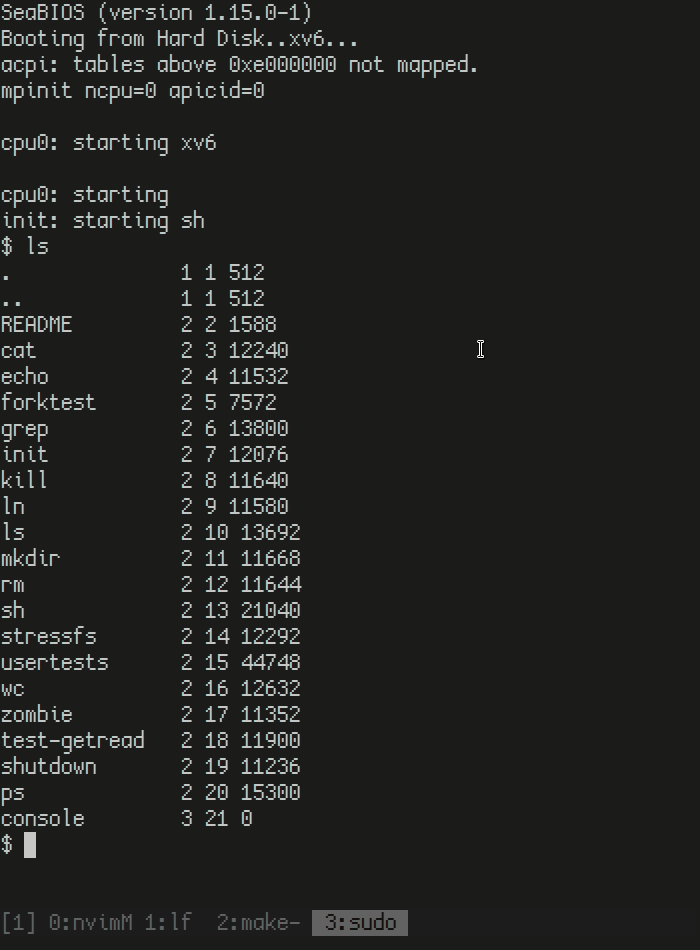
\includegraphics[width=0.7\textwidth]{assets/xv6-start.png}}
    \end{center}
    \caption{Το λειτουργικό σύστημα τρέχει μέσα στον QEMU emulator.}
    \label{fig:xv6-start}
\end{figure}

Η πρώτη διεργασία που εκτελείται είναι η \src{init} η οποία με τη σειρά της εκτελεί ένα shell.
Εδώ μπορείτε να γράψετε εντολές όπως σε ένα τερματικό. Γράψτε την εντολή \src{ls} για να δείτε 
τα αρχεία που βρίσκονται μέσα στο file-system. Μπορείτε να εκτελείται προγράμματα γράφοντας απλά το όνομά τους. 

Εξοικοιωθείτε με τις διαθέσιμες λειτουργίες του λειτουργικού. Ο πηγαίος κώδικας κάθε μίας από τις εφαρμογές αυτές βρίσκεται στον φάκελο \src{user}.

Προς το παρών, δεν υπάρχει τρόπος να απενεργοποιήσετε το σύστημά σας μέσα από αυτή τη γραμμή εντολών.

\section{Ασκήσεις}

\begin{question}
    Διαλέξτε ένα από τα προγράμματα χρήστη στον φάκελο \src{user}. Εξηγήστε τη λειτουργία του κάνοντας συγκεκριμένες αναφορές στα system calls που καλούνε.
\end{question}

\begin{question}
    Δημιουργήστε ένα πρόγραμμα χρήστη για το xv6.

    Μέσα στο φάκελο \src{user}, δημιουργήστε ένα αρχείο με ό'τι όνομα θέλετε. Εκεί, γράψτε ένα πρόγραμμα
    σε γλώσσα \src{C} το οποίο θα κάνει κάτι χρήσιμο. Δώστε προσοχή 
    σε ποιες συναρτήσεις έχετε πρόσβαση. Εδώ, δεν μπορείτε να χρησιμοποήσετε τη βασική βιβλιοθήκη που έχει δημιουργηθεί για το xv6 (\src{ulib}).

    Έπειτα, επεξεργαστείτε κατάλληλα το αρχείο \src{Makefile} ώστε να προστεθεί το πρόγραμμα στο image του xv6 κατά την κατασκευή του (πρέπει να προσθέσετε το όνομα του προγράμματός σας στη λίστα \src{USER\_PROGS}).

    Εκτλέστε \src{make qemu} και χρησιμοποιήστε το πρόγραμμα που δημιουργήσατε μέσα στο xv6.

    \begin{info}[Σημείωση:]
        Μπορείτε να βρείτε τις συναρτήσεις στις οποίες έχετε πρόσβαση σε περιβάλλον χρήστη στο αρχείο \src{include/user.h}.
    \end{info}

\end{question}

\begin{question}
    Αναζητώντας μέσα στον πηγαίο κώδικα του xv6, βρείτε την 
    κλήση συστήματος \src{uptime}.

    \begin{enumerate}
        \item Βρείτε όλα τα σημεία του κώδικα του πυρήνα στα οποία γίνεται αναφορά σε αυτή.
        \item Εξηγήστε την υλοποίησή της.
    \end{enumerate}
\end{question}

\begin{question}
    Βρείτε τη συνάρτηση μέσα στον kernel κώδικα όπου τελικά εκτελούνται οι system calls.
    Καταγράψτε τη σειρά των ενεργειών που γίνονται όταν καλείται ένα system call.
\end{question}

\begin{question}
    Προσθέστε μία κλήση συστήματος η οποία θα επιστρέφει τον αγαπημένο σας αριθμό.
    Η κλήση που θα φτιάξετε πρέπει να έχει το εξής πρωτότυπο: \src{int getfavnum(void)}.
    Μία τέτοια κλήση δεν έχει κανέναν πρακτικό σκοπό αφού δεν εκμεταλεύεται κάποια πληροφορία ή 
    πόρο που κατέχει το λειτουργικό σύστημα. Στόχος εδώ είναι να κατανοήσουμε τον τρόπο με τον οποίο
    προστίθενται κλήσεις συστήματος στο xv6.
\end{question}

\begin{question}
    Προσθέστε μία κλήση συστήματος η οποία θα εκτελεί λειτουργία \textquote{shutdown}. 
    Η κλήση που θα φτιάξετε πρέπει να έχει το εξής πρωτότυπο: \src{void halt(void)}.
    Έπειτα, φτιάξτε ένα πρόγραμμα χρήστη με όνομα \src{shutdown} το οποίο θα καλεί την κλήση συστήματος που φτιάξατε, ώστε 
    χρήστες του xv6 να μπορούν πλέον να κάνουν shutdown το σύστημα χωρίς να χρειάζεται να το κάνουν από το host μηχάνημα.

    Σε αυτή τη κλήση συστήματος θα πρέπει να επικοινωνήσετε άμεσα με το hardware της εικονικής μηχανής (στην περίπτωσή μας το QEMU).
    Για την απενεργοποίηση του συστήματος το hardware περιμένει σε κάποια συγκεκριμένγ διεύθυνση (port) να υπάρξει μία συγκεκριμένη 
    τιμή. Οι αριθμοί για αυτά τα δύο ορίζονται από τον κατασκευαστή.
    Οδηγίες για την τιμή που πρέπει να στείλετε σε ποια πόρτα έχουν καταγραφεί για διάφορους emulators \href{https://wiki.osdev.org/Shutdown}{εδώ}.
    Εξηγήστε τη λειτουργία της συνάρτησης \src{outw} την οποία θα χρησιμοποιήσετε.

    \begin{info}[Σημείωση:]
        Η συνάρτηση \src{outw} είναι ήδη υλοποιημένη στο xv6 και βρίσκεται στο αρχείο \src{include/x86.h}.
    \end{info}
\end{question}

\begin{question}
    Προσθέστε μία κλήση συστήματος η οποία θα επιστρέφει το πόσες φορές έχει εκτελεστεί μία 
    συγκεκριμένη κλήση συστήματος η οποία θα περνιέται σαν όρισμα.
    Η κλήση που θα φτιάξετε πρέπει να έχει το εξής πρωτότυπο: \src{int getcount(int syscall)}.
\end{question}

\begin{question}
    Προσθέστε μία κλήση συστήματος η οποία θα τερματίζει μια τυχαία διεργασία.

    Θα χρειαστεί να προσθέσετε μία \href{https://wiki.osdev.org/Random_Number_Generator#Pseudorandom_number_generators}{γεννήτρια τυχαίων αριθμών} στο kernel.

    \begin{info}[Σημείωση:]
        Για να σκοτώσετε μία διεργασία δωθέντος ενός συγκεκριμένου PID
        μπορείτε να χρησιμοποιήσετε την κλήση συστήματος \src{kill}.
    \end{info}
\end{question}


\printbibliography

\end{document}
